\newpage
\noindent
\textbf{Beispiel 3} \\ \\
a)
\vspace{-15pt}
\usetikzlibrary{arrows}
\begin{figure}[h]
	\centering
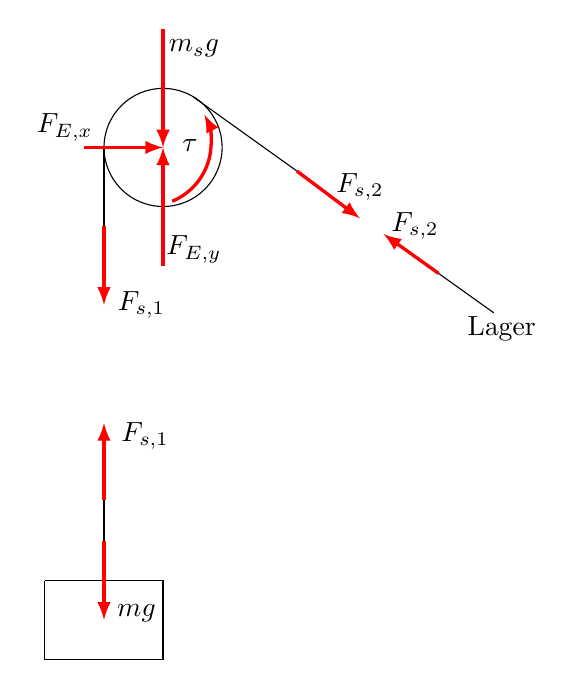
\begin{tikzpicture}
\draw (-3.5,-1) -- (-3.5,-2) -- (-2,-2) -- (-2,-1) -- (-3.5,-1);
\draw (-2.75,-1) -- (-2.75,0.5);
\draw [-latex][red,very thick](-2.75,0.0232) -- (-2.75,1.0);
\draw[-latex][red,very thick](-2.75,-0.5) -- (-2.75, -1.5);
\draw (-2.3377,-1.4121) node {\( mg\)} ;
\draw (-2.228,0.8364) node {\( F_{s,1}\)};
\draw (-1.62,5.145) -- (-0.3,4.2);
\draw  (-2,4.5) circle (0.75);
\draw (-2.75,4.5) -- (-2.75,3.5);
\draw [-latex][red,very thick](-2.75,3.5) -- (-2.75,2.5);
\draw [-latex][red,very thick] (-3,4.5) -- (-2,4.5);
\draw [latex-][red,very thick]  (-2,4.5) -- (-2,6);
\draw [latex-][red,very thick]  (-2,4.5) -- (-2,3);
\draw [-latex][red,very thick](-1.8834,3.8167) arc (-67.5126:26.8608:0.8);
\node at (-2.2741,2.505) {\(F_{s,1}\)};
\node at (-1.6074,3.205) {\( F_{E,y}\)};
\node at (-3.249,4.755) {\(F_{E,x}\)};
\node at (-1.6074,5.755) {\(m_sg\)};
\node at (-1.6574,4.5217) {\( \tau\)};
\draw [-latex][red,very thick] (-0.3,4.2) --(0.5,3.6);
\node at (0.5,4) {\( F_{s,2}\)};
\draw [latex-][red,very thick](0.8,3.4) -- (1.5,2.9);
\draw (1.5,2.9) -- (2.2,2.4);
\node at (1.2,3.5) {\(F_{s,2}\)};
\node at (2.3,2.2) {Lager};
\end{tikzpicture}
\end{figure}
\\ 
Nun müssen die Gleichgewichtsbedingungen für diesen Schnitt bestimmt werden. Diese lauten hier
\begin{align*}
	&\sum M_E = 0: \\
	&\tau -F_{s,2}r + F_{s,1}r = 0 \\
	\\
	&\sum F_x = 0: \\
	&F_{E,x} + F_{s,2}\sin\left(\frac{\pi}{4}\right) = 0 \\
	&F_{E,x} + \frac{F_{s,}}{\sqrt{2}}= 0 \\
	\\
	&\sum F_y = 0:\\
	&F_{E,y} - F_{s,1} - F_{s,2}\sin\left(\frac{\pi}{4}\right) - m_sg = 0\\
	&F_{E,y} - F_{s,1} - \frac{F_{s,2}}{\sqrt{2}} - m_sg = 0
\end{align*}
\newpage
Nun werden die Kräfte im Punkt E und die Seilkräfte berechnet.
\begin{align*}
	&F_{s,1} = mg \\
	\\
	&\tau -F_{s,2}r + F_{s,1}r = 0 \\
	& F_{s,2} r = \tau + m g r \\
	& F_{s,2} = mg + \frac{\tau}{r} \\
	\\
	&F_{E,x} + \frac{F_{s,2}}{\sqrt{2}}= 0 \\
	&F_{E,x} + \frac{mg}{\sqrt{2}} + \frac{\tau}{r\sqrt{2}} = 0 \\
	&F_{E,x} = - \frac{mg}{\sqrt{2}} - \frac{\tau}{r\sqrt{2}} \\
	\\
	&F_{E,y} - F_{s,1} - \frac{F_{s,2}}{\sqrt{2}} - m_sg = 0 \\
	&F_{E,y} - mg - \frac{mg}{\sqrt{2}} - \frac{\tau}{r\sqrt{2}} - m_sg = 0 \\
	&F_{E,y} = mg \frac{\sqrt{2} + 1}{\sqrt{2}} + \frac{\tau}{r\sqrt{2}} + m_sg
\end{align*}
b)
\begin{figure}[h]
	\centering
\begin{tikzpicture}[scale = 1.5]
\draw (-0.5,0.5) -- (-2,1.5) -- (-0.5,1.5);
\draw [red,very thick][-latex](-3.5,1.5) -- (-2,1.5);
\node at (-3.5,1) {\( F_{B,x}\)};
\draw (-2,1.5) -- (-2,-2.5) -- (-0.5,-2.5);
\draw [red,very thick][-latex](-2,0) -- (-2,1.5); 
\node at (-1.5,0.5) {\(F_{B,y}\)};
\draw [red,very thick][-latex](-3.5,-2.5) -- (-2,-2.5);
\node at (-3.5,-2) {\(F_A\)};
\end{tikzpicture}
\end{figure}
\newpage
Nun werden analog wie in a) die Gleichgewichtsbedingungen aufgestellt.
\begin{align*}
	&\sum M_A = 0: \\
	& F_{B,x}h + F_{E,y} \left(a + b\right) -fa = 0 \\
	& F_{B,x} = - F_{E,y}\frac{a+b}{h} + f\frac{a}{h} \\%Fehler in der Musterlösung
	\\
	&\sum F_x = 0:\\
	&F_{B,x} + F_A +F_{E,x} = 0\\
	&-F_{E,y}\frac{a + b}{h} + f \frac{a}{h} + F_A + F_{E,x} = 0 \\
	&F_A = F_{E,y}\frac{a + b}{h} - f\frac{a}{h} - F_{E,x}  \\
	\\
	&\sum F_y = 0: \\
	&F_{B,y} + F_{E,y} - f = 0 \\
	&F_{B,y} = f - F_{E,y}
\end{align*}
\textbf{ACHTUNG}: Die Ergebnisse in der Musterlösung vom ACIN sind nicht korrekt.\\ \\
c)
\begin{figure}[h]
\centering
\begin{tikzpicture}[scale = 1.5]
\draw (-0.5,0.5) -- (-2,1.5) -- (-0.5,1.5);
\draw [red,very thick][-latex](-3.5,1.5) -- (-2,1.5);
\node at (-3.5,1) {\( F_{B,x}\)};
\draw [blue,very thin](-2,1.5) -- (1.5,1.5);
\draw [blue,very thin](-2,1.5) -- (0.7,-0.3);
\draw [blue,thick][latex-latex](0.4,-0.1) arc (-33.5006:0:2.9);
\node at (1.1,0.6) {\(\alpha\)};
\draw (-2,1.5) -- (-2,-2.5) -- (-0.5,-2.5);
\draw [red,very thick][-latex](-2,0) -- (-2,1.5); 
\node at (-1.5,0.5) {\(F_{B,y}\)};
\draw [red,very thick][-latex](-3.5,-2.5) -- (-2,-2.5);
\node at (-3.5,-2) {\(F_A\)};
\draw [red,very thick][-latex](-1,-2.5) -- (0.5,-2.5);
\node at (-0.5,-2) {\(F_2\)};
\draw [red,very thick][-latex](-1,1.5) -- (0,1.5);
\node at (-0.5,2) {\(F_4\)};
\draw [red,very thick][-latex](-0.8,0.7) -- (-0.2,0.3);
\node at (0,0.5) {\(F_3\)};
\end{tikzpicture}
\end{figure}
\newpage
Es müssen wieder die Gleichgewichtsbedingungen aufgestellt werden. Diese lauten hier
\begin{align*}
	&\alpha = \arctan\left(\frac{h}{a}\right) \\
	&\sum M_B = 0: \\
	&F_Aa + F_2 a = 0 \\
	&F_2 = -F_A \\
	\\
	&\sum F_y = 0: \\
	&F_{B,y} - F_3 \sin\alpha = 0 \\
	&F_3 = \frac{F_{B,y}}{\sin\alpha} \\
	\\
	&\sum F_x = 0: \\
	&F_2 + F_4 + F_3 \cos\alpha + F_{E,x}= 0 \\
	&F_4 = - F_2 - F_{B,y}\frac{\cos\alpha}{\sin\alpha} - F_{E,x}\\
	&F_4 = F_A - \frac{F_{B,y}}{\tan\alpha} - F_{E,x}
\end{align*}